%%% use 10pt options with the asme2ej format
\documentclass[10pt,cleanfoot]{asme2ej}

\usepackage{graphicx} %% for loading jpg figures
\usepackage{amsmath}

%% The class has several options
%  onecolumn/twocolumn - format for one or two columns per page
%  10pt/11pt/12pt - use 10, 11, or 12 point font
%  oneside/twoside - format for oneside/twosided printing
%  final/draft - format for final/draft copy
%  cleanfoot - take out copyright info in footer leave page number
%  cleanhead - take out the conference banner on the title page
%  titlepage/notitlepage - put in titlepage or leave out titlepage
%  
%% The default is oneside, onecolumn, 10pt, final

\title{Thermodynamic Analysis of a Regenerative \\
Reheat Rankine Cycle with a Secondary Loop}

%%% first author
\author{Shane Riley
    \affiliation{
	Undergraduate, Mechanical Engineering\\
	Swanson School of Engineering\\
	Department of Mechanical Engineering and Materials Science\\
	University of Pittsburgh, Pittsburgh, PA 15261, USA\\
    Email: shane.riley@pitt.edu
    }	
}

%%% second author
%%% remove the following entry for single author papers
%%% add more entries for additional authors
\author{Gabriel Vogel
    \affiliation{
	Undergraduate, Mechanical Engineering\\
	Swanson School of Engineering\\
	Department of Mechanical Engineering and Materials Science\\
	University of Pittsburgh, Pittsburgh, PA 15261, USA\\
        Email: gtv2@pitt.edu
    }
}

\begin{document}

\maketitle    

%%%%%%%%%%%%%%%%%%%%%%%%%%%%%%%%%%%%%%%%%%%%%%%%%%%%%%%%%%%%%%%%%%%%%%
\begin{abstract}
{\it 
The Rankine Cycle is fundamental to the operation of utility-scale power plants. While the simplest configuration of the cycle employs only four devices (pump, turbine, boiler, condenser), such a cycle leaves additional efficiency on the table. 
Greater efficiency can be achieved by adding reheat processes, feedwater heaters, and an Organic Rankine Cycle with a lower boiling point fluid. These additions increase the cost and complexity of the cycle, but also increase the efficiency. At the utility-scale, the latter is vastly more important. To analyze and optimize a system with a closed feedwater heater (C.F.H.), open feedwater heater (O.F.H.), reheat, and Organic Rankine Cycle (ORC), a script is presented based upon thermodynamic laws, project constraints, and guiding assumptions. This script is run using the Engineering Equation Solver (EES) and a number of input parameters, and outputs a measure of overall thermal efficiency. Using the model as a guide, an optimal set of state variables is reached for maximum thermal efficiency.
}
\end{abstract}

%%%%%%%%%%%%%%%%%%%%%%%%%%%%%%%%%%%%%%%%%%%%%%%%%%%%%%%%%%%%%%%%%%%%%%
\begin{nomenclature}
\entry{$P$}{Pressure of fluid [kPa].}
\entry{$T$}{Temperature of fluid [C].}
\entry{$x$}{Quality of fluid [-]. When superheated or subcooled, the quality is defined as 100 [-] or -100 [-], respectively.}
\entry{$s$}{Real specific entropy of fluid  [kJ/kg-K].}
\entry{$s_{ideal}$}{Ideal specific entropy of fluid  [kJ/kg-K].}
\entry{$h$}{Real specific enthalpy of fluid [kJ/kg].}
\entry{$h_{ideal}$}{Ideal specific enthalpy of fluid [kJ/kg].}
\entry{$m_{main}$}{Mass flow of main line in steam system [kg/s].}
\entry{$m_{hex}$}{Mass flow of refrigerant loop [kg/s].}
\entry{$y$}{Mass flow fraction released to the CFH [-].}
\entry{$z$}{Mass flow fraction released to the OFH [-].}
\entry{$\eta_{th}$}{Overall thermal efficiency [-].}
\entry{$\eta_{pump}$}{Isentropic efficiency of pumps [-].}
\entry{$\eta_{turbine}$}{Isentropic efficiency of turbines [-].}
\entry{$Q$}{Thermal power transferred through a device [kW].}
\entry{$W$}{Work power transferred through a device [kW].}
\entry{$HEX$}{Heat Exchanger.}
\entry{$C.F.H.$}{Closed Feedwater Heater.}
\entry{$O.F.H.$}{Open Feedwater Heater.}
\entry{$ORC$}{Organic Rankine Cycle.}
\end{nomenclature}

%%%%%%%%%%%%%%%%%%%%%%%%%%%%%%%%%%%%%%%%%%%%%%%%%%%%%%%%%%%%%%%%%%%%%%
\section{Introduction}

\begin{figure}[t]
\begin{center}
\setlength{\unitlength}{0.012500in}%
\begin{picture}(115,35)(255,545)
\thicklines
\put(255,545){\framebox(115,35){}}
\put(275,560){Carnot and Rankine}
\end{picture}
\end{center}
\caption{Carnot and Rankine Cycles}
\label{figure_ASME} 
\end{figure}

Modern society owes itself to the study of thermodynamics, and specifically the Rankine Cycle. Standard of living depends on products made at high-scale and low-cost, and this type of production relies on cheap and accessible energy. The easiest way that humanity has found to produce energy in bulk is by using thermodynamic cycles. As such, it seems no coincidence that most innovations in thermodynamics occurred right before and during the Second Industrial Revolution [1]. The quantities of energy necessary to move humanity forward depended on an understanding of thermodynamics. While other forms of utility-scale power generation have evolved today (Photovoltaics, hydro, wind, etc.), the vast majority of power generation is still done using thermal power plants and thermodynamic cycles [1].

In order to generate work in a thermal power plant, thermodynamic cycles utilize a temperature differential created by a fuel (coal, gas, or radioactive material in a reactor). To maximize the work per heat generated (thermal efficiency), careful consideration must be taken in the selection of the cycle. The Carnot Theorem provides guidance by predicting an absolute maximum of thermal efficiency [1].

The Rankine Cycle, named after Scottish engineer William Rankine, uses the phase change of a working fluid to create isobaric processes during heating and cooling [1]. That, combined with roughly isentropic processes at the pump and turbine, makes the T-S diagram of the Rankine Cycle closely mimic that of the Carnot Cycle, resulting in decent thermal efficiency. While this is the case, there are ways to increase the efficiency further. The analysis presented uses three methods: A secondary loop, feedwater heaters, and a reheat process. Using all of these additional methods at once vastly increases the complexity of the cycle, requiring higher levels of analysis in order to maximize thermal efficiency.

% Figure of carnot and rankine cycles

%%%%%%%%%%%%%%%%%%%%%%%%%%%%%%%%%%%%%%%%%%%%%%%%%%%%%%%%%%%%%%%%%%%%%%
\section{Methodology}

To perform an efficiency optimization of state variables and mass flow rates, the Engineering Equation Solver (EES) serves as a useful tool. EES provides simple lookups on state information, and can solve a system easily given enough relations are supplied. Additionally, EES allows for modulating inputs for optimization using parameter tables.

\subsection{Constraints}

As per the project description, the following constraints must be followed:

\begin{enumerate}
\item
The secondary loop will use R-134a
\item
Maximum turbine inlet P = 25 [MPa] and T = 600 [C]
\item
Minimum turbine quality of 90\%
\item
Maximum reheat temperature of T = 600 [C]
\item
Pumps cannot pump any vapor
\item
Ambient temperature of T = 25 [C]
\item
Minimum temperature differential for condenser, heat exchanger, and closed feedwater heater of 15 [C]
\item
Isentropic efficiencies of pumps and turbines as 60\% and 85\%, respectively
\end{enumerate}

Additionally, the first and second laws of thermodynamics should not be violated by our analysis. The only processes that decrease entropy must be ones that remove heat from the working fluid, and the sum of heats and works in and out should be equal to 0. These two laws provide useful assertions for the analysis.

\subsection{Thermodynamic Assumptions}

To simplify the analysis, the following assumptions will be made:
\begin{enumerate}
\item
Gravitational potential and kinetic energies are small relative to the internal energies of the working fluids, and can be ignored.
\item
All plumbing between devices contains fluid of constant state (i.e. no friction from fluid flow that would increase entropy).
\item
Condensers, boilers, heat exchangers and feedwater heaters are isobaric devices.
\item
The steam trap is an isenthalpic device.
\item
The closed feedwater heater, boiler, and heat exchanger lose no heat to the environment.
\end{enumerate}

\subsection{Calculating Heats and Works}

\begin{figure}[t]
\begin{center}
\setlength{\unitlength}{0.012500in}%
\begin{picture}(115,35)(255,545)
\thicklines
\put(255,545){\framebox(115,35){}}
\put(275,560){State Numbers}
\end{picture}
\end{center}
\caption{State Numbers}
\label{figure_ASME} 
\end{figure}

The power moving into or out of the working fluid can be measured as a difference in specific enthalpies multiplied by the mass flow rate of the fluid and the fraction of the total mass flow (dictated by y, z, and their complements). This is reasonable given the assumptions made in the analysis. Whether the power constitutes work or heat depends on the device being analyzed.

In the EES script, power direction is handled such that all values of Q and W come out as positive, given basic assumptions about which way energy should be flowing. That way, a negative sign in any work or heat quantity raises alarm. The proper signage is handled when calculating net work and thermal efficiency. Examples are shown below:

\begin{equation}
W_{turbine,LP2} = m_{main} * (1-y-z) * (h[12] - h[13])
\label{Turbine work out}
\end{equation}

\begin{equation}
W_{pump,HP} = m_{main} * (h[6] - h[5])
\label{Pump work in}
\end{equation}

\begin{equation}
Q_{boiler,1} = m_{main} * (h[8] - h[7])
\label{Boiler heat in}
\end{equation}

\begin{equation}
Q_{out} = m_{hex} * (h[17] - h[14])
\label{Condenser heat out}
\end{equation}

\begin{equation}
Q_{hex} = m_{hex} * (h[16] - h[15])
\label{Heat across exchangers}
\end{equation}

The heat exchanger heat will be equal for each side, and the closed feedwater heater operates as a heat exchanger. The reheat portion of the boiler is defined as $Q_{boiler,2}$.

\subsection{Isobaric Devices}

For a device that is assumed isobaric, the states across the device are assigned equal pressure. An example is shown below:

\begin{equation}
P[14] = P[17]
\label{Isobaric device}
\end{equation}

For the open feedwater heater, there are four states with equal pressure.

\subsection{Isenthalpic Trap}

The steam trap is isenthalpic. The relation is intuitive:

\begin{equation}
h[3] = h[4]
\label{Isobaric device}
\end{equation}

\subsection{Open Feedwater Heater}

In addition to operating at a constant pressure, the O.F.H. will experience no change in enthalpy. As such, we can relate the enthalpies entering and exiting the O.F.H. using mass flow fractions and specific enthalpies:

\begin{equation}
(z * h[12]) + ((1-y-z) * h[2]) + (y * h[4]) = h[5]
\label{O.F.H. enthalpies}
\end{equation}

\subsection{Inefficiencies of Pumps and Turbines}

Using two state variables at the inlet and pressure at the outlet, it is possible to use isentropic efficiency to find outlet state information. To do this, specific entropy is determined at the input. Then, ideal enthalpy at the outlet is determined assuming ideal entropy. Finally, the real enthalpy at the outlet is determined using the isentropic efficiency. This final relation varies between pumps and turbines:

\begin{equation}
\eta_{pump} = \frac{h[5] - h_{ideal}[6]}{h[5] - h[6]}
\label{Pump entropy}
\end{equation}

\begin{equation}
\eta_{turbine} = \frac{h[8] - h[9]}{h[8] - h_{ideal}[9]}
\label{Turbine entropy}
\end{equation}

\subsection{Known-Goods for Optimization}

With fundamental relations established, additional parameters can be set based on thermodynamic intuition:

\begin{enumerate}
\item
Heat flow across a temperature differential produces entropy that scales with the size of the differential. As such, an optimal system will use the minimum allowable temperature differences for HEX/C.F.H./condenser operation. The outlet temperatures are set with a 15 [C] difference (the condenser is set to 15 [C] above ambient).
\item
It is wasteful to cool working fluid beyond the saturation line. As such, the qualities for all three pump inlets are set to 0 [-].
\item
Using the maximum temperature differential for the entire system is optimal (raises Carnot efficiency). As such, the first turbine inlet state is set to maximum allowable temperature and pressure (superheat).
\item
The maximum reheat temperature is optimal for the main loop, as it drops the heat removal (hex) pressure.
\item
In order to maximize the heat addition pre-boiler, the y-fraction should dump as much heat through the C.F.H. as possible. The y-fraction quality after the C.F.H. is set to 0 [-].
\item
For the ORC, it is ideal to not superheat the refrigerant vapor. The pre-turbine refrigerant quality is set to 1 [-].
\item
Mass flow rate of the main loop will simply scale heats and works evenly, resulting in the same overall efficiency. For simplicity, the mass flow for the water is set to 1 [kg/s].
\end{enumerate}

\subsection{Optimization of Remaining Parameters}

From this point, there remain 4 input parameters to determine a solution (in addition to many thermodynamic state variable function calls).

In the final analysis, the following variables are chosen for optimization:

\begin{enumerate}
\item
Pressure at the C.F.H. (P[9])
\item
Pressure at the reheat section of the boiler (P[10])
\item
Pressure of the O.F.H. (P[12])
\item
Pressure at HEX (water-side) (P[13])
\end{enumerate}

The first two parameters are optimized in tandem while the latter two are set to 200 and 100 [kPa], respectively. Once an ideal set of the first two parameters is reached, the O.F.H. pressure and then the HEX pressure are optimized.

%%%%%%%%%%%%%%%%%%%%%%%%%%%%%%%%%%%%%%%%%%%%%%%%%%%%%%%%%%%%%%%%%%%%%%
\section{Results and Discussion}


\begin{figure}[t]
\begin{center}
\setlength{\unitlength}{0.012500in}%
\begin{picture}(115,35)(255,545)
\thicklines
\put(255,545){\framebox(115,35){}}
\put(275,560){Table of States}
\end{picture}
\end{center}
\caption{Table of States}
\label{figure_ASME} 
\end{figure}

\begin{figure}[t]
\begin{center}
\setlength{\unitlength}{0.012500in}%
\begin{picture}(115,35)(255,545)
\thicklines
\put(255,545){\framebox(115,35){}}
\put(275,560){Final TS diagram}
\end{picture}
\end{center}
\caption{Table of States}
\label{figure_ASME} 
\end{figure}

%%%%%%%%%%%%%%%%%%%%%%%%%%%%%%%%%%%%%%%%%%%%%%%%%%%%%%%%%%%%%%%%%%%%%%
\section{Conclusions}

Following the methodology prescribed leads to a thermal efficiency of $\eta_{th} = 0.423 [-]$, a C.F.H. flow fraction of $y = 0.082 [-]$, and a O.F.H. flow fraction of $z = 0.078 [-]$. Under these specifications, the ORC runs with 14.8 times the mass-flow of the main cycle. The following four input pressures are:

\begin{enumerate}
\item
Pressure at the C.F.H: 1500 [kPa]
\item
Pressure at the reheat: 1500 [kPa]
\item
Pressure of the O.F.H: 340 [kPa]
\item
Pressure at HEX (water-side): 35 [kPa]
\end{enumerate}

Based on the constraints, assumptions, and known-goods established in the model, efficiency is maximized at about a zero pressure-drop between the C.F.H. and the reheat. Therefore, an optimized Rankine cycle of the assigned structure requires no second high pressure turbine. Removing the device would likely decrease the implementation/maintenance costs and remove a point of failure from the cycle. Moving forward, further consideration should likely be taken into maximum allowable mass-flow rates, in order to determine whether the ORC flow speed predicted my the model is truly reasonable. Additionally, a cost analysis could be performed to weigh the cost of additional devices against the gains of additional efficiency.

\begin{acknowledgment}
Special thanks go to Tyler Zinn and Josh Myers for their help in troubleshooting our thermodynamic model, discussing useful source material, and revealing various EES features to us.
\end{acknowledgment}


%%%%%%%%%%%%%%%%%%%%%%%%%%%%%%%%%%%%%%%%%%%%%%%%%%%%%%%%%%%%%%%%%%%%%%
%\section{Figures}
%\label{sect_figure}
%
%All figures should be positioned at the top of the page where possible.  All figures should be numbered consecutively and centered under the figure as shown in Fig.~\ref{figure_ASME}. All text within the figure should be no smaller than 7~pt. There should be a minimum two line spaces between figures and text. The number of a referenced figure or table in the text should be preceded by Fig.\ or Tab.\ respectively unless the reference starts a sentence in which case Fig.\ or Tab.\ should be expanded to Figure or Table.
%
%
%%%%%%%%%%%%%%%%%%%%%%%%%%%%%%%%%%%%%%%%%%%%%%%%%%%%%%%%%%%%%%%%%%%%%%%
%%%%%%%%%%%%%%%%% begin figure %%%%%%%%%%%%%%%%%%%
%\begin{figure}[t]
%\begin{center}
%\setlength{\unitlength}{0.012500in}%
%\begin{picture}(115,35)(255,545)
%\thicklines
%\put(255,545){\framebox(115,35){}}
%\put(275,560){Beautiful Figure}
%\end{picture}
%\end{center}
%\caption{The caption of a single sentence does not have period at the end}
%\label{figure_ASME} 
%\end{figure}
%%%%%%%%%%%%%%%%% end figure %%%%%%%%%%%%%%%%%%% 
%%%%%%%%%%%%%%%%%%%%%%%%%%%%%%%%%%%%%%%%%%%%%%%%%%%%%%%%%%%%%%%%%%%%%%%
%
%In the following subsections, I have inserted figures that have been provided by authors in order to demonstrate what to avoid.  In each case the authors provided figures that are 3.25in wide and 600dpi in the .tif graphics format.  The papers containing these figures have been held from production due to their poor quality. 
%
%%%%%%%%%%%%%%%%%%%%%%%%%%%%%%%%%%%%%%%%%%%%%%%%%%%%%%%%%%%%%%%%%%%%%%%
%\subsection{The 1st Example of Bad Figure}
%
%%%%%%%%%%%%%%%%% begin figure %%%%%%%%%%%%%%%%%%%
%%%% 3.34in is the maximum width you can have for a figure
%\begin{figure} 
%\centerline{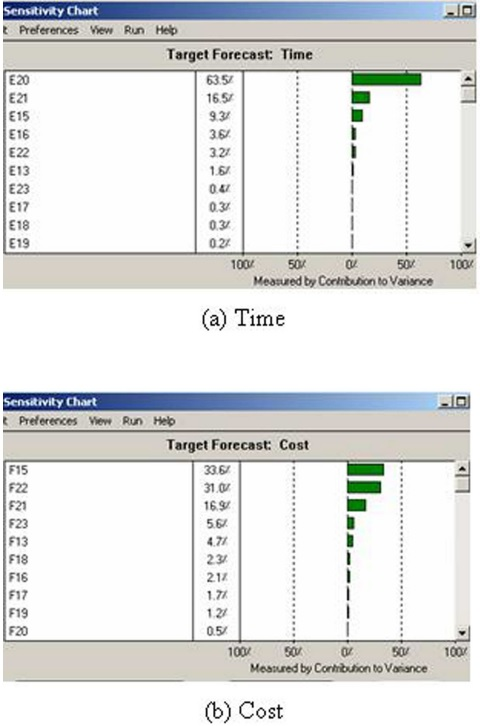
\includegraphics[width=3.34in]{figure/FMANU_MD_05_1107_11.jpg}}
%\caption{Example taken from a paper that was held from production because the image quality is poor.  ASME sets figures captions in 8pt, Helvetica Bold.}
%\label{fig_example1.jpg}
%\end{figure}
%%%%%%%%%%%%%%%%% end figure %%%%%%%%%%%%%%%%%%%
%
%In order to place the figure in this template using MSWord, select Insert Picture from File, and use wrapping that is top and bottom. Make sure the figure is 3.25in wide.
% 
%Figure~`\ref{fig_example1.jpg}
%was taken from a recent paper that was held from publication, because the text is fuzzy and unreadable. It was probably obtained by taking a screen shot of the computer output of the authors software. This means the original figure was 72dpi (dots per inch) on a computer screen. There is no way to improve the quality such a low resolution figure.
% 
%In order to understand how poor the quality of this figure is, please zoom in slightly, say to 200\%. Notice that while the font of the paper is clear at this size, the font in the figures is fuzzy and blurred. It is impossible to make out the small symbol beside the numbers along the abscissa of the graph. Now consider the labels Time and Cost. They are clearly in fonts larger that the text of the article, yet the pixilation or rasterization, associated with low resolution is obvious. This figure must be regenerated at higher resolution to ensure quality presentation.
%
%The poor quality of this figure is immediately obvious on the printed page, and reduces the impact of the research contribution of the paper, and in fact detracts from the perceived quality of the journal itself.
%
%
%
%%%%%%%%%%%%%%%%%%%%%%%%%%%%%%%%%%%%%%%%%%%%%%%%%%%%%%%%%%%%%%%%%%%%%%%
%\subsection{The 2nd Example of Bad Figure}
%
%%%%%%%%%%%%%%%%% begin figure %%%%%%%%%%%%%%%%%%%
%\begin{figure} 
%\centerline{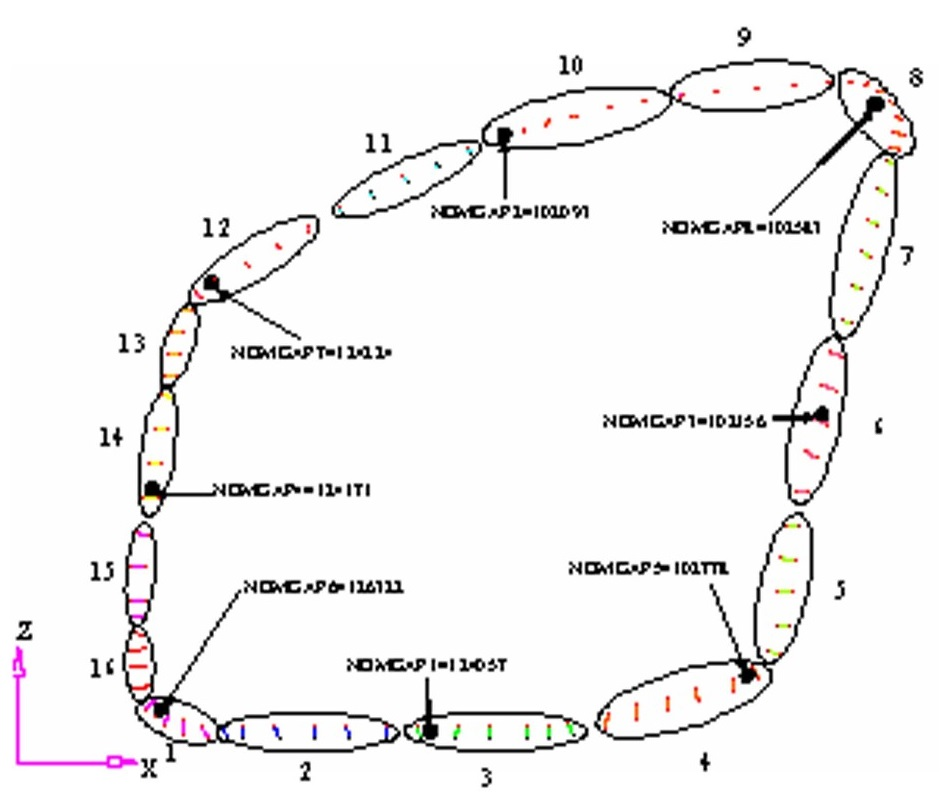
\includegraphics[width=3.34in]{figure/FMANU_MD_05_1272_5.jpg}}
%\caption{While this figures is easily readable at a double column width of 6.5in, when it is shrunk to 3.25in column width the text is unreadable.   This paper was held from production.}
%\label{fig_example2.jpg}
%\end{figure}
%%%%%%%%%%%%%%%%% end figure %%%%%%%%%%%%%%%%%%%
%
%Figure~\ref{fig_example2.jpg}
%demonstrates a common problem that arises when a figure is scaled down fit a single column width of 3.25in.  The original figure had labels that were readable at full size, but become unreadable when scaled to half size.  This figure also suffers from poor resolution as is seen in the jagged lines the ovals that form the chain.
%
%This problem can be addressed by increasing the size of the figure to a double column width of 6.5in, so the text is readable.  But this will not improve the line pixilation, and a large low resolution figure is less desirable than a small one.  This also significantly expands the length of the paper, and may cause it to exceed the JMD nine page limit.  Additional pages require page charges of \$200 per page.  It is best to regenerate the figure at the resolution that ensures a quality presentation.
%
%
%%%%%%%%%%%%%%%%%%%%%%%%%%%%%%%%%%%%%%%%%%%%%%%%%%%%%%%%%%%%%%%%%%%%%%%
%\subsection{The 3rd Example of Bad Figure}
%%%%%%%%%%%%%%%%% begin figure %%%%%%%%%%%%%%%%%%%
%\begin{figure} 
%%\centerline{\psfig{figure=figure/FMANU_MD_04_1274_13.ps,width=3.34in}}
%\centerline{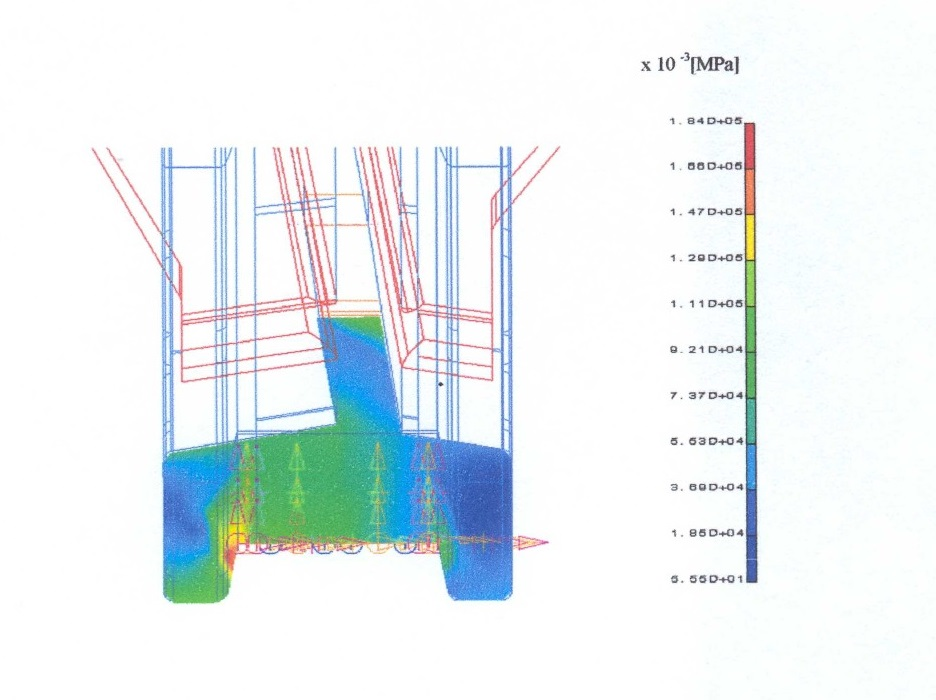
\includegraphics[width=3.25in]{figure/FMANU_MD_04_1274_13.jpg}}
%\caption{Another example of a figure with unreadable text.  Even when the paper was expanded to double column width the text as shown in Fig.~\ref{fig_example4.jpg} was of such low quality that the paper was held from production.}
%\label{fig_example3.jpg}
%\end{figure}
%%%%%%%%%%%%%%%%% end figure %%%%%%%%%%%%%%%%%%%
%
%%%%%%%%%%%%%%%%% begin figure %%%%%%%%%%%%%%%%%%%
%%%% the maximum width in double column is 6.85in
%\begin{figure*} 
%\centerline{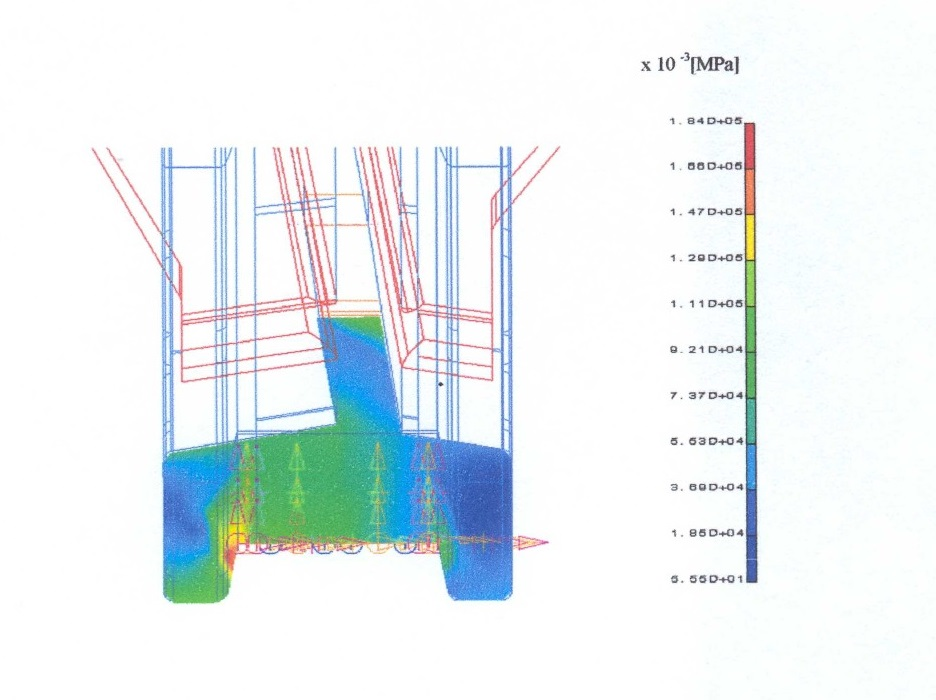
\includegraphics[width=6.85in]{figure/FMANU_MD_04_1274_13.jpg}}
%\caption{A figure expanded to double column width the text from Figure~\ref{fig_example3.jpg}}
%\label{fig_example4.jpg}
%\end{figure*}
%%%%%%%%%%%%%%%%% end figure %%%%%%%%%%%%%%%%%%%
%An author provided the high resolution image 
%in Fig.~\ref{fig_example3.jpg}
%that was sized to a single column width of 3.25in.  Upon seeing the poor quality of the text, the publisher scaled the image to double column width as shown in Fig.~\ref{fig_example4.jpg} 
%at which point it took half of a page.  The publisher went on to do this for all eight figures generating four pages of figures that the author did not expect. ASME stopped production of the paper even with the larger figures due to the pixilation of the font.
%
%Clearly the text in this figure is unreadable, and it is doubtful that the author can print the output in a way that it is readable.  This is a problem that the author must solve, not the publisher. 
%
%As you might expect, I have many more examples, but in the end the author is the best judge of what is needed in each figure.  ASME simply requires that the image meet a minimum standard for font and line quality, specifically the font should be the appropriate size and not be blurred or pixilated, and that lines should be the appropriate weight and have minimal, preferably no, pixilation or rasterization.
%
%
%%%%%%%%%%%%%%%%%%%%%%%%%%%%%%%%%%%%%%%%%%%%%%%%%%%%%%%%%%%%%%%%%%%%%%%
%\section{Tables}
%
%%%%%%%%%%%%%%%%%%%%%%%%%%%%%%%%%%%%%%%%%%%%%%%%%%%%%%%%%%%%%%%%%%%%%%%
%%%%%%%%%%%%%%%% begin table   %%%%%%%%%%%%%%%%%%%%%%%%%%
%\begin{table}[t]
%\caption{Figure and table captions do not end with a period}
%\begin{center}
%\label{table_ASME}
%\begin{tabular}{c l l}
%& & \\ % put some space after the caption
%\hline
%Example & Time & Cost \\
%\hline
%1 & 12.5 & \$1,000 \\
%2 & 24 & \$2,000 \\
%\hline
%\end{tabular}
%\end{center}
%\end{table}
%%%%%%%%%%%%%%%%% end table %%%%%%%%%%%%%%%%%%% 
%%%%%%%%%%%%%%%%%%%%%%%%%%%%%%%%%%%%%%%%%%%%%%%%%%%%%%%%%%%%%%%%%%%%%%%
%
%All tables should be numbered consecutively  and centered above the table as shown in Table~\ref{table_ASME}. The body of the table should be no smaller than 7 pt.  There should be a minimum two line spaces between tables and text.
%
%
%%%%%%%%%%%%%%%%%%%%%%%%%%%%%%%%%%%%%%%%%%%%%%%%%%%%%%%%%%%%%%%%%%%%%%%
%\section{Citing References}
%
%%%%%%%%%%%%%%%%%%%%%%%%%%%%%%%%%%%%%%%%%%%%%%%%%%%%%%%%%%%%%%%%%%%%%%%
%The ASME reference format is defined in the authors kit provided by the ASME.  The format is:
%
%\begin{quotation}
%{\em Text Citation}. Within the text, references should be cited in  numerical order according to their order of appearance.  The numbered reference citation should be enclosed in brackets.
%\end{quotation}
%
%The references must appear in the paper in the order that they were cited.  In addition, multiple citations (3 or more in the same brackets) must appear as a `` [1-3]''.  A complete definition of the ASME reference format can be found in the  ASME manual \cite{asmemanual}.
%
%The bibliography style required by the ASME is unsorted with entries appearing in the order in which the citations appear. If that were the only specification, the standard {\sc Bib}\TeX\ unsrt bibliography style could be used. Unfortunately, the bibliography style required by the ASME has additional requirements (last name followed by first name, periodical volume in boldface, periodical number inside parentheses, etc.) that are not part of the unsrt style. Therefore, to get ASME bibliography formatting, you must use the \verb+asmems4.bst+ bibliography style file with {\sc Bib}\TeX. This file is not part of the standard BibTeX distribution so you'll need to place the file someplace where LaTeX can find it (one possibility is in the same location as the file being typeset).
%
%With \LaTeX/{\sc Bib}\TeX, \LaTeX\ uses the citation format set by the class file and writes the citation information into the .aux file associated with the \LaTeX\ source. {\sc Bib}\TeX\ reads the .aux file and matches the citations to the entries in the bibliographic data base file specified in the \LaTeX\ source file by the \verb+\bibliography+ command. {\sc Bib}\TeX\ then writes the bibliography in accordance with the rules in the bibliography .bst style file to a .bbl file which \LaTeX\ merges with the source text.  A good description of the use of {\sc Bib}\TeX\ can be found in \cite{latex, goosens} (see how two references are handled?).  The following is an example of how three or more references \cite{latex, asmemanual,  goosens} show up using the \verb+asmems4.bst+ bibliography style file in conjunction with the \verb+asme2ej.cls+ class file. Here are some more \cite{art, blt, ibk, icn, ips, mts, mis, pro, pts, trt, upd} which can be used to describe almost any sort of reference.
%
%%%%%%%%%%%%%%%%%%%%%%%%%%%%%%%%%%%%%%%%%%%%%%%%%%%%%%%%%%%%%%%%%%%%%%%
%\section{Conclusions}
%The only way to ensure that your figures are presented in the ASME Journal of Mechanical Design in the way you feel is appropriate and meets the requirement for quality presentation is for you to prepare a double column version of the paper in a form similar to that used by the Journal.
%
%This gives you the opportunity to ensure that the figures are sized appropriately, in particular that the labels are readable and match the size of the text in the journal, and that the line weights and resolutions have no pixilation or rasterization.  Poor quality figures are immediately obvious on the printed page, and this detracts from the perceived quality of the journal.
%
%I am pleased to provide advice on how to improve any figure, but this effort must start with a two-column version of the manuscript. Thank you in advance for your patience with this effort, it will ensure quality presentation of your research contributions.

%%%%%%%%%%%%%%%%%%%%%%%%%%%%%%%%%%%%%%%%%%%%%%%%%%%%%%%%%%%%%%%%%%%%%%
% The bibliography is stored in an external database file
% in the BibTeX format (file_name.bib).  The bibliography is
% created by the following command and it will appear in this
% position in the document. You may, of course, create your
% own bibliography by using thebibliography environment as in

\begin{thebibliography}{12}
\bibitem{itemreference} {\em Rankine Cycle - Steam Turbine Cycle.}
{\em Nuclear Power.}
{Nuclear Power for Everybody.}
\end{thebibliography}

% Here's where you specify the bibliography style file.
% The full file name for the bibliography style file 
% used for an ASME paper is asmems4.bst.
\bibliographystyle{asmems4}

% Here's where you specify the bibliography database file.
% The full file name of the bibliography database for this
% article is asme2e.bib. The name for your database is up
% to you.
\bibliography{asme2e}
\end{document}
